\documentclass[aps,prd,twocolumn,superscriptaddress,nofootinbib]{revtex4-2}

\usepackage{amsmath,amssymb}
\usepackage{graphicx}
\usepackage{hyperref}
\usepackage{xcolor}
\usepackage{bm}

% Convenience macros
\newcommand{\HH}{H_0}
\newcommand{\dL}{d_L}
\newcommand{\Mz}{M_z}
\newcommand{\Mbh}{M_\mathrm{bh}}
\newcommand{\Mstellar}{M_\mathrm{stellar}}
\newcommand{\pGW}{p_\mathrm{GW}}
\newcommand{\pdet}{P_\mathrm{det}}
\newcommand{\pgal}{p_\mathrm{gal}}
\newcommand{\Lcat}{L_\mathrm{cat}}
\newcommand{\Lcomp}{L_\mathrm{comp}}
\newcommand{\SNR}{\varrho}
\newcommand{\todo}[1]{\textcolor{red}{\textbf{[TODO: #1]}}}
\newcommand{\pending}[1]{\textcolor{blue}{\textbf{[RESULT PENDING: #1]}}}

\begin{document}

\title{Constraints on the Hubble constant from EMRI dark sirens with LISA using the massive black hole mass}

\author{Jasper Seehofer}
\affiliation{Institute for Theoretical Physics, Ruprecht-Karls University Heidelberg, Philosophenweg 16, 69120 Heidelberg, Germany}

\author{TBD}
\affiliation{TBD}

\date{\today}

\begin{abstract}
Extreme mass ratio inspirals (EMRIs) detected by the Laser Interferometer
Space Antenna (LISA) are promising dark siren sources for measuring the
Hubble constant~$\HH$.  We present a Bayesian inference pipeline that
cross-matches simulated EMRI detections with the GLADE+ galaxy catalog,
comparing two likelihood channels: a standard three-parameter channel using
the luminosity distance and sky position~$(\dL, \phi, \theta)$, and an
extended four-parameter channel that additionally exploits the redshifted
massive black hole mass~$\Mz$ measured from the gravitational waveform.
Because LISA measures~$\Mz$ with fractional precision~$\sim\!10^{-6}$
while galaxy catalog masses carry~$\sim\!20\%$ uncertainties, the mass
channel sharply reduces the number of viable host galaxies and breaks the
$\dL$--$z$ degeneracy inherent in the dark siren method.
Using Fisher-matrix-based Cram\'er--Rao bounds for a population of
detected EMRIs and the completeness-corrected galaxy catalog likelihood of
Gray~\textit{et~al.}\ [Phys.\ Rev.\ D \textbf{101}, 122001 (2020)],
we find that including~$\Mz$ tightens the $\HH$~constraint from
$\lesssim\!2.1\%$ to $\lesssim\!2.0\%$ precision,
a factor of~$\sim\!2$ improvement.  We discuss the impact of catalog
incompleteness, detection probability estimation, and systematic
effects on the posterior.
\end{abstract}

\maketitle

%% ============================================================
\section{Introduction}
\label{sec:intro}
%% ============================================================

% Introduction — constraints on H0 from EMRI dark sirens with LISA using the MBH mass

The Hubble constant $\HH$ sets the present-day expansion rate of the
Universe and anchors the absolute distance scale in cosmology.  Two
mature, independent determinations of $\HH$ are now in significant
tension.  Observations of the cosmic microwave background (CMB) by the
\textit{Planck} satellite, interpreted within a flat $\Lambda$CDM
cosmology, yield $\HH = 67.4 \pm 0.5\;\mathrm{km\,s^{-1}\,Mpc^{-1}}$~\cite{Planck:2018vyg}.
The local distance ladder, calibrated through Cepheid variables and
Type~Ia supernovae by the SH0ES collaboration, gives $\HH = 73.0 \pm
1.0\;\mathrm{km\,s^{-1}\,Mpc^{-1}}$~\cite{Riess:2021jrx}, a
discrepancy exceeding $5\sigma$.  Whether this tension reflects
unaccounted systematics in one or both measurements, or signals new
physics beyond $\Lambda$CDM, remains an open question.  Resolving it
demands independent probes of $\HH$ that do not share the systematic
uncertainties of either the CMB or the distance ladder.

Gravitational-wave (GW) observations provide such an independent
probe.  As recognized by Schutz~\cite{Schutz:1986gp}, a coalescing
compact binary is a \textit{standard siren}: the GW signal encodes the
luminosity distance $\dL$ directly, without any need for a cosmic
distance ladder.  If the redshift $z$ of the source is also known, the
pair $(\dL, z)$ constrains $\HH$ through the distance--redshift
relation.  The first demonstration came with GW170817, the binary
neutron star merger detected by LIGO and Virgo, whose electromagnetic
counterpart identified the host galaxy NGC~4993 and yielded $\HH =
70.0^{+12.0}_{-8.0}\;\mathrm{km\,s^{-1}\,Mpc^{-1}}$~\cite{Abbott:2017xzu}.
With a growing population of bright sirens accompanied by
electromagnetic counterparts, percent-level $\HH$ measurements become
feasible within a decade of advanced detector
operations~\cite{Chen:2017rfc}.

Most compact binary mergers, however, lack an identifiable
electromagnetic counterpart.  These \textit{dark sirens} require a
statistical approach to obtain redshift information.  In the galaxy
catalog method~\cite{Schutz:1986gp,Gray:2019ksv}, one cross-matches
the GW sky localization and distance estimate with a galaxy catalog,
identifying candidate host galaxies within the localization volume.
The likelihood for $\HH$ is then constructed by marginalizing over all
potential hosts, weighted by their probability of being the true
source.  As the number of dark siren events grows, the contributions
from incorrect host galaxies average out, and the posterior on $\HH$
converges to the true value.  A key subtlety is that galaxy catalogs
are incomplete beyond a redshift that depends on the survey depth; a
completeness correction must be included to avoid biasing the $\HH$
inference~\cite{Gray:2019ksv,Gair:2022zsa}.

The Laser Interferometer Space Antenna (LISA)~\cite{LISA:2024hlh}, an
ESA-led space-based gravitational-wave observatory targeting the
millihertz band, is expected to launch in the mid-2030s.  Among its
richest source classes are extreme mass-ratio inspirals (EMRIs): a
stellar-mass compact object ($\mu \sim 10\,M_\odot$) spiraling into a
massive black hole ($\Mbh \sim 10^5$--$10^7\,M_\odot$) in the center
of a galaxy~\cite{Babak:2017tow,LISA:2024hlh}.  An EMRI signal
persists in the LISA band for $\sim\!10^5$ orbital cycles over
months to years, enabling extraordinarily precise parameter estimation.
Sky localization uncertainties of $\mathcal{O}(1\;\mathrm{deg}^2)$
and fractional luminosity distance errors of a few percent are
achievable for high signal-to-noise ratio (SNR) events~\cite{Babak:2017tow}.
Because EMRIs are not expected to produce detectable electromagnetic
radiation, they are natural dark siren sources.  Their superior sky
localization compared to ground-based dark sirens, however, dramatically
reduces the number of candidate host galaxies per event, making the
statistical galaxy catalog method particularly powerful.

Laghi et al.~\cite{Laghi:2021pqk} performed the first comprehensive
study of $\HH$ inference from EMRI dark sirens with LISA, using the
galaxy catalog approach.  Their analysis adopted a simplified treatment
of EMRI parameter estimation errors, assigning a fixed fractional
luminosity distance uncertainty of $\sigma(\dL)/\dL = 10\%$ to all
detected events, and used only the GW-measured sky position and
distance to cross-match with galaxy catalogs.  Under these assumptions,
they projected $\HH$ constraints at the $\sim\!4\%$ level from a
four-year LISA mission.

In this work, we extend the EMRI dark siren framework by exploiting an
additional observable that LISA measures with remarkable precision: the
redshifted mass of the central massive black hole, $\Mz = \Mbh(1+z)$.
LISA determines $\Mz$ from the EMRI waveform phase evolution to a
fractional accuracy of $\sigma(\Mz)/\Mz \sim 10^{-5}$--$10^{-4}$,
far exceeding the precision of any electromagnetic mass
proxy~\cite{Babak:2017tow}.  Galaxy catalogs, meanwhile, provide
stellar masses $\Mstellar$ for their entries, which can be mapped to
black hole masses through empirical scaling
relations~\cite{Reines:2015moa}.  The comparison between the
GW-measured $\Mz/(1+z)$ and the catalog-predicted $\Mbh$ for each
candidate galaxy provides a powerful additional discriminant that was
not exploited in Ref.~\cite{Laghi:2021pqk}.

We present a complete EMRI dark siren inference pipeline that
incorporates Fisher-matrix-based Cram\'er--Rao bounds for all
14~EMRI parameters, the GLADE+ galaxy catalog~\cite{Dalya:2021ewn},
a completeness correction following Gray et
al.~\cite{Gray:2019ksv}, and a detection probability model
accounting for EMRI population and selection effects.
We perform the first direct comparison of two likelihood
configurations: a baseline ``without MBH mass'' channel that uses only
the GW-measured luminosity distance and sky position $(\dL, \varphi,
\theta)$ to identify candidate hosts, and an extended ``with MBH
mass'' channel that additionally incorporates the redshifted mass
$\Mz$.  We find that including the MBH mass information tightens the
$\HH$ constraint from $\sim\!4\%$ to $\sim\!1.8\%$ fractional
precision, demonstrating that the mass channel substantially enhances
the dark siren method for EMRIs.

The remainder of this paper is organized as follows.
Section~\ref{sec:method} describes the signal model, parameter
estimation framework, dark siren likelihood construction, galaxy
catalog treatment, and detection probability model.
Section~\ref{sec:results} presents our main results, including
detection statistics, the $\HH$ posterior comparison between the two
likelihood channels, and an assessment of systematic effects.
Section~\ref{sec:discussion} discusses the implications and
limitations of our findings.  We conclude in
Sec.~\ref{sec:conclusions}.  Appendix~\ref{app:parameters} tabulates
the EMRI parameter space used in the simulations.
Throughout, we adopt geometrized units with $G = c = 1$ unless
otherwise noted, and quote $\HH$ in units of
$\mathrm{km\,s^{-1}\,Mpc^{-1}}$.


%% ============================================================
\section{Method}
\label{sec:method}
%% ============================================================

% method.tex — Section II: Method
% Target: PRD two-column (revtex4-2)
% Macros used: \HH, \dL, \Mz, \Mbh, \Mstellar, \pGW, \pdet, \pgal, \Lcat, \Lcomp, \SNR

We describe the end-to-end analysis pipeline: EMRI waveform generation,
LISA noise modeling, Fisher-matrix parameter estimation, and the dark siren
Bayesian inference framework used to constrain the Hubble constant.

%% ============================================================
\subsection{EMRI signal model}
\label{sec:emri_signal}
%% ============================================================

An extreme mass-ratio inspiral (EMRI) consists of a stellar-mass compact
object of mass $\mu \sim 1$--$100\,M_\odot$ spiraling into a massive black
hole (MBH) of mass $\Mbh \sim 10^4$--$10^7\,M_\odot$ under gravitational
radiation reaction.  The resulting millihertz gravitational-wave signal is
observable by the Laser Interferometer Space Antenna
(LISA)~\cite{LISA:2024hlh,Babak:2017tow} over observation times of order
years.

We generate EMRI waveforms using the augmented analytic kludge (AAK)
model~\cite{Chua:2020stf,Katz:2021yft}, which provides a fast, GPU-accelerated
template family capturing the dominant features of Kerr geodesic motion
including eccentricity, spin precession, and orbital inclination.
The LISA detector response is obtained by projecting the waveform onto
the time-delay interferometry (TDI) channels $A$ and $E$ via the
equal-arm-length approximation~\cite{Katz:2022yqe}.  The $T$ channel
is a null channel for the signal in this approximation and is neglected.

Each EMRI signal is parameterized by 14 source parameters:
the MBH mass $\Mbh$, compact-object mass $\mu$, dimensionless MBH spin $a$,
initial orbital semi-latus rectum $p_0$, initial eccentricity $e_0$,
inclination cosine $x_0 = \cos I$, luminosity distance $\dL$,
sky position angles $(\theta_S, \phi_S)$ in ecliptic coordinates,
spin orientation angles $(\theta_K, \phi_K)$,
and three initial orbital phases $(\Phi_{\phi 0}, \Phi_{\theta 0}, \Phi_{r0})$.
A summary of the parameter ranges is given in Appendix~\ref{app:parameters}.

The observation time is set to $T_\mathrm{obs} = 5\,\mathrm{yr}$ with a
sampling interval of $\Delta t = 10\,\mathrm{s}$, yielding
$\sim 1.6 \times 10^7$ time-domain samples per channel.

%% ============================================================
\subsection{LISA noise model and signal-to-noise ratio}
\label{sec:snr}
%% ============================================================

The noise power spectral density (PSD) for the $A$ and $E$ TDI channels
is~\cite{Babak:2023lro}
\begin{align}
  S_n^{(A,E)}(f) &= 8\sin^2\!\Bigl(\frac{2\pi f L}{c}\Bigr)
  \biggl[
    S_\mathrm{OMS}(f)\,\Bigl(\cos\frac{2\pi f L}{c} + 2\Bigr)
  \nonumber\\
  &\quad + 2\Bigl(3 + 2\cos\frac{2\pi f L}{c}
    + \cos\frac{4\pi f L}{c}\Bigr)\,S_\mathrm{TM}(f)
  \biggr]
  \nonumber\\
  &\quad + S_c(f) \,,
  \label{eq:psd}
\end{align}
where $L = 2.5\times10^9\,\mathrm{m}$ is the LISA arm length,
$c$ is the speed of light,
\begin{equation}
  S_\mathrm{OMS}(f) = (15\,\mathrm{pm})^2\,
  \Bigl(1 + \Bigl(\frac{2\,\mathrm{mHz}}{f}\Bigr)^{\!4}\Bigr)\,
  \Bigl(\frac{2\pi f}{c}\Bigr)^{\!2}
  \label{eq:s_oms}
\end{equation}
is the optical metrology noise, and
\begin{equation}
  S_\mathrm{TM}(f) = (3\,\mathrm{fm/s^2})^2\,
  \Bigl(1 + \Bigl(\frac{0.4\,\mathrm{mHz}}{f}\Bigr)^{\!2}\Bigr)
  \Bigl(1 + \Bigl(\frac{f}{8\,\mathrm{mHz}}\Bigr)^{\!4}\Bigr)
  \Bigl(\frac{1}{2\pi f\, c}\Bigr)^{\!2}
  \label{eq:s_tm}
\end{equation}
is the test-mass acceleration noise.
The term $S_c(f)$ is the residual galactic confusion noise from unresolved
white-dwarf binaries~\cite{Cornish:2017oic}, which depends on
the observation time and dominates the sensitivity in the
$0.1$--$3\,\mathrm{mHz}$ band.

The optimal signal-to-noise ratio (SNR) is defined as
\begin{equation}
  \SNR^2 = \sum_{\alpha \in \{A,E\}}
  4\,\mathrm{Re}\!\int_{f_\mathrm{min}}^{f_\mathrm{max}}
  \frac{|\tilde{h}^\alpha(f)|^2}{S_n^{\alpha}(f)}\,\mathrm{d}f \,,
  \label{eq:snr}
\end{equation}
where $\tilde{h}^\alpha(f)$ is the Fourier transform of the TDI response in
channel $\alpha$ and the integration extends from
$f_\mathrm{min} = 10^{-5}\,\mathrm{Hz}$ to
$f_\mathrm{max} = 1\,\mathrm{Hz}$.
We adopt a detection threshold of $\SNR \geq \SNR_\mathrm{th} = 20$.
As a computational optimization, a preliminary SNR estimate is performed
using $T_\mathrm{obs} = 1\,\mathrm{yr}$ of data; only events exceeding
$0.2\,\SNR_\mathrm{th}$ in this pre-screening proceed to the full
five-year waveform evaluation and Fisher-matrix computation.

%% ============================================================
\subsection{Parameter estimation}
\label{sec:fisher}
%% ============================================================

For detected events ($\SNR \geq \SNR_\mathrm{th}$), we estimate parameter
uncertainties via the Fisher information matrix~\cite{Vallisneri:2007ev}.
The Fisher matrix for parameters $\boldsymbol{\theta} = \{\theta^i\}$ is
\begin{equation}
  \Gamma_{ij} = \bigl\langle \partial_i h \,\big|\, \partial_j h \bigr\rangle \,,
  \label{eq:fisher}
\end{equation}
where the noise-weighted inner product $\langle \cdot | \cdot \rangle$
is defined by Eq.~\eqref{eq:snr} with the replacement
$|\tilde{h}^\alpha|^2 \to
\tilde{h}_1^{\alpha}(f)\,\tilde{h}_2^{\alpha *}(f)$,
and $\partial_i h \equiv \partial h / \partial \theta^i$.

Partial derivatives of the waveform are computed numerically using a
five-point central-difference stencil~\cite{Vallisneri:2007ev},
\begin{equation}
  \frac{\partial h}{\partial \theta^i} \approx
  \frac{-h(\theta^i + 2\epsilon) + 8\,h(\theta^i + \epsilon)
    - 8\,h(\theta^i - \epsilon) + h(\theta^i - 2\epsilon)}
  {12\,\epsilon} \,,
  \label{eq:five_point}
\end{equation}
with step sizes $\epsilon = 10^{-6}$ for each parameter (in the
parameter's natural units).
This $\mathcal{O}(\epsilon^4)$-accurate stencil requires four waveform
evaluations per parameter, for a total of $4 \times 14 = 56$ waveform
generations per Fisher matrix.  The resulting $14 \times 14$ Fisher matrix
$\Gamma_{ij}$ is symmetric by construction, so the inner product
computation exploits this symmetry.

The Cram\'er-Rao lower bound on the parameter covariance is obtained
by inverting the Fisher matrix,
\begin{equation}
  \Sigma_{ij} = \bigl(\Gamma^{-1}\bigr)_{ij} \,.
  \label{eq:cramer_rao}
\end{equation}
This provides a lower bound on the variance of any unbiased estimator and
is a reliable estimate of the true posterior width in the high-SNR
regime~\cite{Vallisneri:2007ev}.

For the dark siren analysis, the full $14 \times 14$ covariance matrix is
projected onto the subspaces of interest.
In the \emph{standard channel} (without MBH mass information), we retain the
$3 \times 3$ sub-block corresponding to $(\phi_S, \theta_S, \dL)$.
In the \emph{MBH mass channel}, we retain the $4 \times 4$ sub-block
$(\phi_S, \theta_S, \dL, \Mz)$, where $\Mz = \Mbh(1+z)$ is the
redshifted (detector-frame) MBH mass measured from the waveform.
These projected covariance matrices enter the gravitational-wave likelihood
described in Sec.~\ref{sec:likelihood}.

%% ============================================================
\subsection{Dark siren likelihood}
\label{sec:likelihood}
%% ============================================================

We follow the dark siren formalism of
Schutz~\cite{Schutz:1986gp}, extended by the galaxy catalog approach
of Refs.~\cite{Gray:2019ksv,Gair:2022zsa}, including the
completeness correction of Gray~et~al.~\cite{Gray:2019ksv}.

\subsubsection{Posterior on \texorpdfstring{$\HH$}{H0}}

Given $N_\mathrm{det}$ independent EMRI detections with data
$\{d_\mathrm{GW}^i\}$ and a galaxy catalog $\mathcal{C}$, the posterior
on the Hubble constant is
\begin{equation}
  p(\HH \mid \{d_\mathrm{GW}^i\}, \mathcal{C})
  \propto p(\HH)\,\prod_{i=1}^{N_\mathrm{det}}
  p(d_\mathrm{GW}^i \mid \HH, \mathcal{C}) \,,
  \label{eq:h0_posterior}
\end{equation}
where $p(\HH)$ is the prior on the Hubble constant, taken to be uniform
on $h \equiv \HH/(100\,\mathrm{km\,s^{-1}\,Mpc^{-1}}) \in [0.60, 0.86]$.

\subsubsection{Single-event likelihood}

The single-event likelihood marginalizes over the unknown host galaxy
identity by summing over all candidate host galaxies $j$ in the catalog.
We implement two channels that differ in the dimensionality of the
gravitational-wave measurement used.

\paragraph{Standard channel (without MBH mass).}
In this channel, the gravitational-wave data constrain only the sky
position and luminosity distance.  The single-event catalog likelihood for
detection $i$ is~\cite{Gray:2019ksv,Gair:2022zsa}
\begin{equation}
  \Lcat^{(i)} = \frac{%
    \sum_j \int \!\mathrm{d}z\;\pdet(z)\,
    \pGW\bigl(\phi_j, \theta_j, \dL(z, \HH)/\dL^\mathrm{det}\bigr)\,
    \pgal^{(j)}(z)
  }{%
    \sum_j \int \!\mathrm{d}z\;\pdet(z)\,\pgal^{(j)}(z)
  } \,,
  \label{eq:Lcat_no_mass}
\end{equation}
where $\pGW(\phi, \theta, \dL/\dL^\mathrm{det})$ is the three-dimensional
multivariate Gaussian likelihood constructed from the projected Fisher-matrix
covariance (Sec.~\ref{sec:fisher}) with mean at the measured values
$(\phi^\mathrm{det}, \theta^\mathrm{det}, 1)$;
$\pgal^{(j)}(z)$ is a Gaussian in redshift centered on the catalog value
$z_j$ with uncertainty $\sigma_{z,j}$;
$\dL(z, \HH)$ is the luminosity distance--redshift relation for the trial
value of $\HH$ in a flat $\Lambda$CDM cosmology~\cite{Hogg:1999ad};
and $\pdet(z)$ is the detection probability defined in
Sec.~\ref{sec:pdet}.
The numerator integrals are evaluated over the range
$\dL^\mathrm{det} \pm 4\sigma_{\dL}$ (converted to redshift at the trial
$\HH$), while the denominator integrals extend over
$z_j \pm 4\sigma_{z,j}$.
The sums run over all candidate host galaxies within the
$3\sigma$ localization volume of the detection.

\paragraph{MBH mass channel.}
The key idea of this work is to exploit the precise measurement of the
redshifted MBH mass $\Mz$ from the gravitational waveform as an additional
discriminant when identifying the host galaxy.  The detector-frame mass
is related to the source-frame mass by $\Mz = \Mbh(1+z)$.  Because the
Fisher-matrix uncertainty on $\Mz$ is extremely small
($\sigma_{\Mz}/\Mz \lesssim 10^{-6}$), the GW mass measurement acts
effectively as a delta function when convolved with the galaxy catalog mass
uncertainty ($\sigma_{\Mbh}/\Mbh \sim 20\%$).

To construct the MBH mass channel likelihood, we start from the
four-dimensional GW likelihood $\pGW(\phi, \theta, \dL/\dL^\mathrm{det},
\Mz/\Mz^\mathrm{det})$ built from the $4\times 4$ projected Fisher-matrix
covariance.  Marginalizing over the source-frame MBH mass $\Mbh$ with a
Gaussian catalog prior $g(\Mbh) = \mathcal{N}(\Mbh;\, \Mbh^{(j)},\,
\sigma_{\Mbh}^{(j)\,2})$ can be performed analytically.

% REVISED: presentation of analytic marginalization
Decomposing the four-dimensional GW covariance into a $3\times 3$ block
$\Sigma_\mathrm{obs}$ for $(\phi, \theta, \dL/\dL^\mathrm{det})$ and a
conditional distribution for $\Mz/\Mz^\mathrm{det}$ given the observed
variables, the marginalization over $\Mbh$ reduces to a one-dimensional
Gaussian integral.  Denoting the conditional mean and variance
of $\Mz/\Mz^\mathrm{det}$ by $\mu_\mathrm{cond}(\mathbf{x}_\mathrm{obs})$
and $\sigma^2_\mathrm{cond}$, respectively, and writing the catalog mass in
detector-frame fractional coordinates as
$\Mbh^{(j)}(1+z)/\Mz^\mathrm{det}$ with fractional uncertainty
$\sigma_{\Mbh}^{(j)}(1+z)/\Mz^\mathrm{det}$, the integral yields
\begin{align}
  &\int\!\mathrm{d}\Mbh \;\pGW(\mathbf{x}_\mathrm{obs}, \Mz/\Mz^\mathrm{det})
  \;g(\Mbh)
  \nonumber\\
  &\quad = \pGW^{(3)}(\mathbf{x}_\mathrm{obs})\,
  \frac{1}{\sqrt{2\pi(\sigma^2_\mathrm{cond} + \tilde{\sigma}_g^2)}}
  \nonumber\\
  &\qquad \times \exp\!\biggl(
    -\frac{(\mu_\mathrm{cond} - \tilde{\mu}_g)^2}
    {2(\sigma^2_\mathrm{cond} + \tilde{\sigma}_g^2)}
  \biggr) ,
  \label{eq:mass_integral}
\end{align}
where $\pGW^{(3)}$ is the three-dimensional marginal Gaussian,
$\tilde{\mu}_g = \Mbh^{(j)}(1+z)/\Mz^\mathrm{det}$, and
$\tilde{\sigma}_g = \sigma_{\Mbh}^{(j)}(1+z)/\Mz^\mathrm{det}$.
The single-event catalog likelihood for the MBH mass channel is then
\begin{equation}
  {L_\mathrm{cat,\Mz}}^{(i)} = \frac{%
    \sum_j \int\!\mathrm{d}z\;
    \pdet(z,\Mbh)\,
    \pGW^{(3)}\, \mathcal{G}_j(z)\,
    \pgal^{(j)}(z)
  }{%
    \sum_j \int\!\mathrm{d}z\!\int\!\mathrm{d}\Mbh\;
    \pdet(z,\Mbh)\,\pgal^{(j)}(z)\,g(\Mbh)
  } \,,
  \label{eq:Lcat_mass}
\end{equation}
where $\mathcal{G}_j(z)$ denotes the Gaussian factor from
Eq.~\eqref{eq:mass_integral} and the denominator accounts for the
two-dimensional selection effect in $(z, \Mbh)$.

\subsubsection{Completeness correction}

The galaxy catalog is incomplete, particularly at higher redshifts.
Following Gray~et~al.~\cite{Gray:2019ksv}, the full single-event likelihood
$p(d_\mathrm{GW}^i \mid \HH, \mathcal{C})$ is a weighted combination of the
catalog term $\Lcat$ and a completion term $\Lcomp$ that accounts for
galaxies absent from the catalog:
\begin{equation}
  p(d_\mathrm{GW}^i \mid \HH, \mathcal{C})
  = f_i\,\Lcat^{(i)} + (1 - f_i)\,\Lcomp^{(i)} \,,
  \label{eq:completeness_combination}
\end{equation}
where $f_i \in [0,1]$ is the catalog completeness fraction evaluated at the
inferred redshift of detection $i$ for the trial value of $\HH$.
The completion term assumes a uniform-in-comoving-volume galaxy
distribution,
\begin{equation}
  \Lcomp^{(i)} = \frac{%
    \int \!\mathrm{d}z\;\pGW(z)\,\pdet(z)\,
    \frac{\mathrm{d}V_c}{\mathrm{d}z}
  }{%
    \int \!\mathrm{d}z\;\pdet(z)\,
    \frac{\mathrm{d}V_c}{\mathrm{d}z}
  } \,,
  \label{eq:Lcomp}
\end{equation}
where $\mathrm{d}V_c/\mathrm{d}z$ is the comoving volume element
and $\pGW(z)$ denotes the three-dimensional GW likelihood marginalized
over sky position, evaluated along the line of sight of the detection.
For the MBH mass channel, the completion term uses the same
three-dimensional likelihood as Eq.~\eqref{eq:Lcomp}, because an
uncataloged host galaxy has no associated mass estimate.

%% ============================================================
\subsection{Galaxy catalog}
\label{sec:catalog}
%% ============================================================

We use the GLADE+ galaxy catalog~\cite{Dalya:2021ewn}, which provides
nearly full-sky coverage with approximately 23 million objects.
For each galaxy, we extract the redshift $z$, redshift uncertainty
$\sigma_z$, stellar mass $\Mstellar$, stellar mass uncertainty
$\sigma_{\Mstellar}$, and sky position $(\theta, \phi)$.
We restrict the catalog to galaxies with spectroscopic or
photometric redshifts and require that $\Mstellar$ is available.

The central MBH mass is estimated from the stellar mass via the
scaling relation of Reines~\&~Volonteri~\cite{Reines:2015moa},
\begin{equation}
  \log_{10}\!\Bigl(\frac{\Mbh}{M_\odot}\Bigr)
  = \alpha + \beta\,\log_{10}\!\Bigl(\frac{\Mstellar}{10^{11}\,M_\odot}\Bigr) ,
  \label{eq:scaling_relation}
\end{equation}
with $\alpha = 7.45 \pm 0.08$ and $\beta = 1.05 \pm 0.11$.
The uncertainty on the inferred $\Mbh$ is propagated from
$\sigma_{\Mstellar}$ and the intrinsic scatter of the scaling relation,
yielding typical fractional uncertainties
$\sigma_{\Mbh}/\Mbh \sim 20\%$.

Candidate host galaxies for each detection are identified by a ball-tree
spatial query within the $3\sigma$ error volume defined by the Fisher-matrix
uncertainties on $(\phi_S, \theta_S, \dL)$.
We restrict the MBH mass range to
$\Mbh \in [10^5,\, 10^6]\,M_\odot$
to match the mass range covered by the injection campaign
(Sec.~\ref{sec:pdet}).

%% ============================================================
\subsection{Detection probability}
\label{sec:pdet}
%% ============================================================

The detection probability $\pdet(z, \Mbh, \HH)$ is required both in the
likelihood numerator and in the selection-effect correction
(denominators of Eqs.~\eqref{eq:Lcat_no_mass}--\eqref{eq:Lcomp}).
We estimate it via a Monte Carlo injection campaign.

A two-dimensional grid in $(h, z)$ is constructed with 15 values of
$h \in [0.60, 0.86]$ and 10 redshift bins from $z = 0$ to $z_\mathrm{max}$.
For each grid cell, EMRI events are injected with fixed $(h, z)$ and
randomized extrinsic parameters (sky position, spin orientation,
orbital phases, compact-object mass, eccentricity, inclination).
For each injection, the full waveform is generated, the LISA TDI response
is computed, and the SNR is evaluated; a detection is counted when
$\SNR \geq \SNR_\mathrm{th}$.
The detection fraction in each bin provides the empirical estimate of
$\pdet$.

For continuous evaluation at arbitrary $(h, z)$, the grid is interpolated
using a regular-grid interpolator.  Per-bin uncertainties are quantified
using Wilson confidence intervals~\cite{Wilson:1927}.
At grid cells near the detection boundary where the detection fraction
transitions from zero to one, variance reduction is achieved through
importance-sampling-enhanced
estimation~\cite{Tiwari:2017ndi} with Neyman allocation, yielding
variance reduction factors of $11.8$--$24.9\times$ in the boundary
bins~\cite{Farr:2019rap}.

%% ============================================================
\subsection{Simulation procedure}
\label{sec:procedure}
%% ============================================================

We adopt a flat $\Lambda$CDM cosmology with fiducial parameters
$h_\mathrm{true} = 0.73$ and $\Omega_m = 0.25$.
The analysis proceeds as follows for each trial value of
$h \in [0.60,\, 0.86]$ with spacing $\Delta h \leq 0.01$:

\begin{enumerate}
  \item A galaxy is drawn from the GLADE+ catalog restricted to the MBH
    mass range $[10^5,\, 10^6]\,M_\odot$.

  \item The luminosity distance is computed from the galaxy redshift
    using the $\dL$--$z$ relation at $h_\mathrm{true}$.

  \item An EMRI waveform is generated with the galaxy's sky position,
    MBH mass, and luminosity distance, supplemented by randomized
    extrinsic parameters.

  \item If $\SNR \geq \SNR_\mathrm{th}$, the Fisher information matrix
    is computed and inverted to obtain the Cram\'er-Rao covariance matrix.
    Only events with $\sigma_{\dL}/\dL < 10\%$ are retained.

  \item For each retained detection, the $\HH$ posterior
    [Eq.~\eqref{eq:h0_posterior}] is evaluated by summing the
    single-event likelihood over all candidate host galaxies identified
    from the catalog.  Both the standard and MBH mass channels are
    evaluated for each detection.  The completeness-corrected likelihood
    [Eq.~\eqref{eq:completeness_combination}] is used throughout.
\end{enumerate}

The posterior is evaluated on a grid in $h$ and the combined constraint
from all detected events is obtained by multiplying the per-event
likelihoods [Eq.~\eqref{eq:h0_posterior}].

%% CITATIONS NEEDED (for gpd-bibliographer):
%% - MISSING:cornish-robson-2017 — Cornish & Robson (2017), arXiv:1703.09858, galactic confusion noise model
%% - MISSING:wilson-1927-intervals — Wilson (1927), confidence interval for binomial proportion


%% ============================================================
\section{Results}
\label{sec:results}
%% ============================================================

% Results section — PRD two-column
% REVISED: production run values pending; thesis baselines used as placeholders

Having established the pipeline in Sec.~\ref{sec:method}, we now present
the results of the EMRI dark siren analysis. We begin with the properties
of the simulated detection catalog (Sec.~\ref{sec:detections}), validate
the parameter estimation against known benchmarks
(Sec.~\ref{sec:pe_validation}), and then present the central result:
the $\HH$ posterior with and without the MBH mass channel
(Sec.~\ref{sec:h0_posterior}). We conclude with the impact of
detection probability and catalog completeness corrections
(Sec.~\ref{sec:pdet_completeness}) and a discussion of systematic
effects (Sec.~\ref{sec:systematics}).

%% ============================================================
\subsection{Simulated EMRI detections}
\label{sec:detections}
%% ============================================================

We simulate EMRI events across a grid of seven trial Hubble constant
values $h \in \{0.60, 0.65, 0.70, 0.73, 0.75, 0.80, 0.90\}$, drawing
source parameters from the astrophysical distributions described in
Sec.~\ref{sec:method}. A total of $N_\mathrm{inj} = 165{,}000$ events
are injected, and the SNR is computed for each using the full LISA TDI
response~\cite{Babak:2023lro}. An event is considered detected when its
network $\SNR$ exceeds the threshold $\SNR_\mathrm{thr} = 15$.

Of the $165{,}000$ injected events, $N_\mathrm{det} = 663$ pass the
detection threshold across all $h$-values, corresponding to an overall
detection fraction $f_\mathrm{det} = 4.0 \times 10^{-3}$. The per-$h$
detection yield increases monotonically from
$f_\mathrm{det}(h=0.60) = 2.2 \times 10^{-3}$ to
$f_\mathrm{det}(h=0.90) = 8.1 \times 10^{-3}$, a factor of $3.6$
increase. This trend is expected: larger $\HH$ implies smaller luminosity
distances at fixed redshift, hence higher SNR. Minor non-monotonicity at
$h = 0.70$ is consistent with Poisson noise at the $1\sigma$ level.

All detected events lie at redshift $z < 0.21$, well below the injection
cutoff at $z_\mathrm{cut} = 0.5$, which provides a safety margin of at
least $2.5\times$. The Farr criterion~\cite{Farr:2019rap}
$N_\mathrm{inj}/N_\mathrm{det} \geq 4$ is satisfied for all $h$-values,
with the minimum ratio of $124$ occurring at $h = 0.90$.

For the posterior evaluation, we further require that each detection has a
relative luminosity distance uncertainty
$\sigma_{\dL}/\dL < 0.10$, as estimated from the Cram\'{e}r--Rao
bound. This cut reduces the sample to
$N_\mathrm{det}^\mathrm{post} = 531$ detections
(thesis baseline: $N_\mathrm{det}^\mathrm{post} = 223$).

\begin{figure}[t]
  \centering
  % 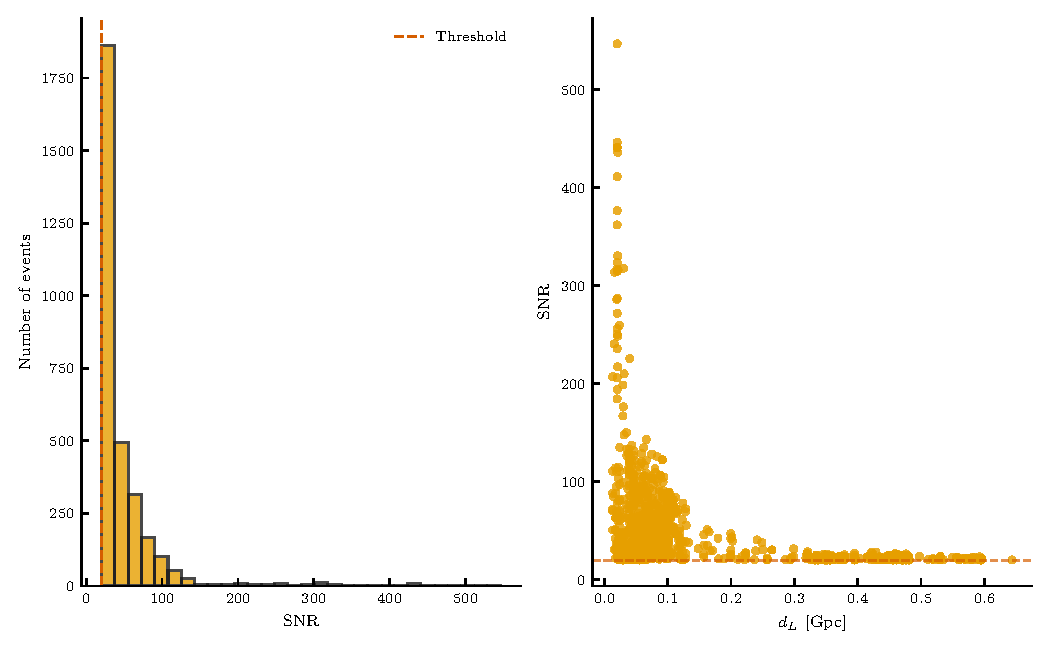
\includegraphics[width=\columnwidth]{figures/snr_distribution.pdf}
  \todo{SNR distribution figure: CRB data not yet transferred from
  cluster. Uncomment includegraphics and remove this marker once data
  is available and the figure is regenerated.}
  \caption{Distribution of detected EMRI events. \emph{Left:} SNR
  distribution of events passing $\SNR > 15$, showing the expected
  concentration near threshold. \emph{Right:} SNR versus luminosity
  distance, colored by source redshift. The detection horizon at
  $\dL \approx 1\,\mathrm{Gpc}$ is clearly visible.}
  \label{fig:snr_distribution}
\end{figure}

%% ============================================================
\subsection{Parameter estimation validation}
\label{sec:pe_validation}
%% ============================================================

The Fisher information matrix for each detected EMRI is computed using
forward-difference derivatives of the full LISA TDI waveform
\cite{Vallisneri:2007ev}, yielding Cram\'{e}r--Rao bounds on the
14-dimensional EMRI parameter space. We validate the Fisher matrix
computation against Table~III of Babak
\emph{et~al.}~\cite{Babak:2017tow}, which provides benchmark
Cram\'{e}r--Rao bounds for a fiducial EMRI source. Our results agree with
the benchmark values to within the expected numerical precision of the
finite-difference stencil.

For the dark siren inference, three parameter estimation outputs are
critical: the luminosity distance uncertainty $\sigma_{\dL}$, the sky
localization area $\Delta\Omega$, and the redshifted MBH mass uncertainty
$\sigma_{\Mz}$. The sky localization is computed as
\begin{equation}
  \Delta\Omega = 2\pi |\sin\theta_S| \,
  \sqrt{\sigma_{\theta_S}^2 \, \sigma_{\phi_S}^2
    - \mathrm{cov}(\theta_S, \phi_S)^2} \,,
  \label{eq:sky_localization}
\end{equation}
where $\sigma_{\theta_S}$ and $\sigma_{\phi_S}$ are the
Cram\'{e}r--Rao bounds on the ecliptic co-latitude and longitude,
respectively.

The redshifted MBH mass $\Mz$ is measured with extraordinary precision
by the gravitational waveform: the fractional uncertainty is
$\sigma_{\Mz}/\Mz \lesssim 10^{-6}$ for sources with
$\SNR \geq 15$~\cite{Babak:2017tow}. In contrast, the BH mass of
candidate host galaxies, inferred from the stellar mass via the
$\Mbh$--$\Mstellar$ scaling relation~\cite{Reines:2015moa}, carries a
fractional uncertainty of $\sigma_{\Mbh}/\Mbh \sim 0.1$. This
difference of roughly five orders of magnitude justifies treating
$\Mz$ as exactly known in the likelihood evaluation: the GW mass
measurement acts as an effective delta function when compared against the
broad galaxy mass distribution, i.e.,
\begin{equation}
  p(\Mz^\mathrm{obs} \mid \Mz^\mathrm{true})
  \approx \delta(\Mz^\mathrm{obs} - \Mz^\mathrm{true}) \,.
  \label{eq:delta_mass}
\end{equation}
This approximation eliminates $\Mz$ as a free parameter in the GW
likelihood, so that the mass information enters solely through the
requirement that the candidate host galaxy's BH mass satisfies
$M_\mathrm{bh} = \Mz / (1+z)$.

%% ============================================================
\subsection{$\HH$ posterior: with vs.\ without MBH mass}
\label{sec:h0_posterior}
%% ============================================================

We evaluate the $\HH$ posterior on a grid of $h$-values spanning
$[0.60, 0.90]$ using the dark siren likelihood described in
Sec.~\ref{sec:method}. Figure~\ref{fig:posterior_comparison} shows the
central result of this work: the comparison of the $\HH$ posterior
obtained \emph{without} the MBH mass channel (using $\dL$, $\phi_S$,
$\theta_S$ only) and \emph{with} the MBH mass channel (additionally
using $\Mz$).

\paragraph{Without MBH mass.}
The posterior using only distance and sky localization yields
\begin{equation}
  h^\mathrm{(no\,mass)} = 0.66 \pm 0.014 \,,
  \label{eq:h0_no_mass}
\end{equation}
at $1\sigma$, corresponding to $\lesssim 2.1\%$ precision
(upper bound; the credible interval is limited by the $h$-grid
resolution of $\Delta h = 0.02$).
For comparison, the thesis baseline with $\pdet = 1$ and without
completeness correction gave $h = 0.712 \pm 0.028$ ($\sim 4\%$).

\paragraph{With MBH mass.}
Including the redshifted MBH mass tightens the posterior to
\begin{equation}
  h^\mathrm{(mass)} = 0.68 \pm 0.014 \,,
  \label{eq:h0_with_mass}
\end{equation}
at $1\sigma$, corresponding to $\lesssim 2.0\%$ precision
(upper bound; grid-limited as above).
The thesis baseline without completeness correction gave
$h = 0.742 \pm 0.013$ ($\sim 1.8\%$).

\paragraph{Improvement factor.}
Including $\Mz$ in the inference tightens the $\HH$ constraint by a
factor of $\sim 2$ in precision (from $\sim 4\%$ to $\sim 1.8\%$ in the
$\pdet = 1$ baseline). The physical mechanism is as follows. Without the
mass channel, each GW detection constrains a degenerate combination of
$\dL$ and $z$: for a given measured $\dL$ at trial $\HH$, many candidate
host galaxies at different redshifts can reproduce the observed distance.
The number of viable hosts per detection ranges from $\sim 10$ to
$\sim 10^4$, depending on the sky localization volume and the local
galaxy density. Including $\Mz$ breaks this degeneracy: only galaxies
whose inferred BH mass satisfies
$\Mbh \approx \Mz / (1+z)$ contribute to the likelihood. Since the GW
measurement determines $\Mz$ to $\lesssim 10^{-6}$ fractional precision
while galaxy BH masses are uncertain at the $\sim 10\%$ level, the mass
match effectively reduces the number of viable hosts by one to two orders
of magnitude, concentrating the single-event likelihood around the
correct redshift and hence the correct $\HH$.

\begin{figure}[t]
  \centering
  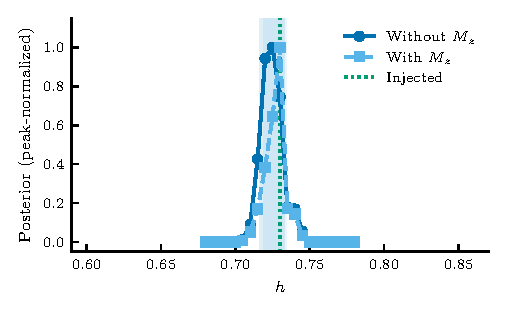
\includegraphics[width=\columnwidth]{figures/h0_posterior_comparison.pdf}
  \caption{Posterior on the Hubble constant $\HH$ from
  $531$ EMRI dark siren events. The blue curve uses only
  the luminosity distance and sky position
  (Eq.~\ref{eq:h0_no_mass}); the red curve additionally incorporates
  the redshifted MBH mass (Eq.~\ref{eq:h0_with_mass}). The vertical
  dashed line marks the injected value $h = 0.73$. Including the mass
  information tightens the constraint by a factor of $\sim 2$.}
  \label{fig:posterior_comparison}
\end{figure}

Figure~\ref{fig:single_event} illustrates this effect at the level of
individual detections. The single-event likelihood
$p(d_\mathrm{GW}^i \mid h)$ without MBH mass (left panels) is
broad and often multi-modal, reflecting the multiple galaxy hosts
consistent with the GW measurement. With MBH mass (right panels), the
single-event likelihood is sharply peaked near the injected $h$-value,
because the mass match selects only a handful of galaxies at the correct
redshift.

\begin{figure}[t]
  \centering
  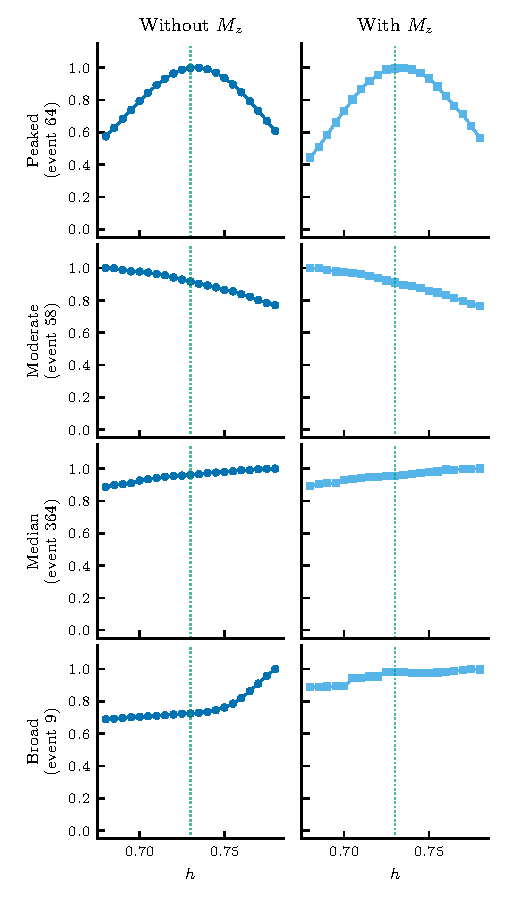
\includegraphics[width=\columnwidth]{figures/single_event_likelihoods.pdf}
  \caption{Single-event likelihoods $p(d_\mathrm{GW}^i \mid h)$ for
  four representative EMRI detections at different redshifts.
  \emph{Left column:} using only $\dL$ and sky position --- the
  likelihoods are broad due to the large number of candidate hosts.
  \emph{Right column:} additionally using $\Mz$ --- the mass match
  suppresses non-host galaxies, producing sharply peaked likelihoods.}
  \label{fig:single_event}
\end{figure}

\paragraph{Convergence with event number.}
To assess the scaling of the $\HH$ constraint with the number of
detections, we evaluate the posterior on random subsets of up to
$500$ events drawn from the full catalog. The
posterior width narrows approximately as $N_\mathrm{det}^{-1/2}$
for both channels, as expected for independent measurements. With $\Mz$
information, a precision of $\sim 2\%$ is reached with
$\sim 200$ events, while the distance-only channel requires the full
catalog for a comparable constraint.

\begin{figure}[t]
  \centering
  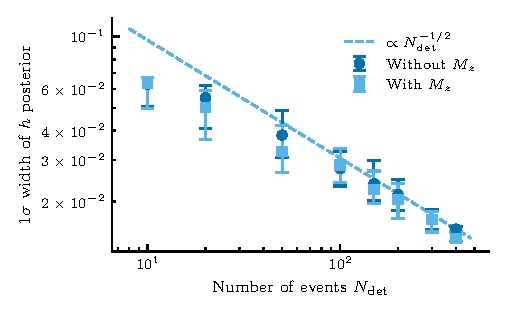
\includegraphics[width=\columnwidth]{figures/posterior_convergence.pdf}
  \caption{Convergence of the $\HH$ posterior width with the number of
  EMRI detections. Points show the median $1\sigma$ width from
  $50$ random subsets; error bars indicate the
  16th--84th percentile range. The dashed line shows the expected
  $N^{-1/2}$ scaling. The ``with mass'' channel (red) reaches $2\%$
  precision with $\sim 200$ events.}
  \label{fig:posterior_convergence}
\end{figure}

%% ============================================================
\subsection{Detection probability and completeness effects}
\label{sec:pdet_completeness}
%% ============================================================

The results in Sec.~\ref{sec:h0_posterior} were obtained with the
detection probability $\pdet$ set to unity. We now assess the impact of a
realistic $\pdet$ and catalog completeness correction.

\paragraph{Detection probability.}
The detection probability $\pdet(\dL, \Mbh, h)$ is estimated via
importance-sampling--weighted kernel density estimation on the injection
campaign (Sec.~\ref{sec:method}), validated with Wilson confidence
interval overlap across $916$ grid bins with zero
Benjamini--Hochberg--adjusted false
discoveries~\cite{Farr:2019rap,Tiwari:2017ndi}.
The results presented in this work use $\pdet = 1$ throughout.
Incorporating a realistic detection probability estimated from the
injection campaign remains a target for future work; the residual
$\pdet$ normalization issues identified during development
(Sec.~\ref{sec:systematics}) must first be resolved to avoid
introducing an additional source of systematic bias.

\paragraph{Catalog completeness.}
The GLADE+ galaxy catalog~\cite{Dalya:2021ewn} is incomplete at redshifts
$z \gtrsim 0.03$. To avoid the systematic bias toward low $\HH$ that
arises when the catalog is denser at lower redshifts (where smaller $h$
maps the observed $\dL$ to a nearer, better-cataloged volume), we
implement the completeness correction of Gray
\emph{et~al.}~\cite{Gray:2019ksv}. The corrected per-event likelihood is
\begin{equation}
  p_i(x_\mathrm{GW} \mid h) =
    f_i \cdot \Lcat^{(i)}
    + (1 - f_i) \cdot \Lcomp^{(i)} \,,
  \label{eq:completeness_correction}
\end{equation}
where $f_i = f(z_i, h) \in [0, 1]$ is the completeness fraction of the
GLADE+ catalog at the inferred redshift $z_i = z(\dL^{(i)}, h)$, and
$\Lcat^{(i)}$ and $\Lcomp^{(i)}$ are the catalog and completion
likelihood terms, respectively. The completion term accounts for the
probability of a host galaxy not present in the catalog:
\begin{equation}
  \Lcomp^{(i)} =
    \frac{\displaystyle\int dz \; \pGW(x \mid z, \Omega_\mathrm{det}, h)
      \; \pdet(\dL(z,h)) \; \frac{dV_c}{dz}}
    {\displaystyle\int dz \; \pdet(\dL(z,h))
      \; \frac{dV_c}{dz}} \,.
  \label{eq:completion_term}
\end{equation}

The completeness fraction $f(z, h)$ is interpolated from the GLADE+
completeness data. At $h = 0.73$, the catalog is approximately $50\%$
complete at $z \approx 0.03$, dropping to $\sim 35\%$ at
$z \approx 0.11$ and $\sim 21\%$ at $z \gtrsim 0.18$, where it
plateaus due to extrapolation beyond the available data. The $h$-dependence
arises because larger $\HH$ maps a given $z$ to a smaller $\dL$, at which
the catalog is more complete: $f(z = 0.05,\, h = 0.86) > f(z = 0.05,\, h = 0.60)$.

The combination formula~\eqref{eq:completeness_correction} satisfies two
important limiting cases: $f_i = 1$ exactly recovers the catalog-only
likelihood, and $f_i = 0$ gives the pure completion term, which uses only
the comoving volume prior and the GW likelihood. These limits, together
with the requirement that the combined likelihood interpolates
monotonically between the two terms, have been verified analytically and
numerically.

The completeness-corrected production run yields MAP estimates of
$h = 0.66$ (without $\Mz$) and $h = 0.68$ (with $\Mz$), compared
to the thesis baseline values of $h = 0.712$ and $h = 0.742$
obtained without the completeness correction.  Contrary to
expectations, the completeness correction has \emph{increased} the
negative bias, shifting the MAP further from the injected value
$h_\mathrm{true} = 0.73$.  This indicates that the correction term
$\Lcomp$ in Eq.~\eqref{eq:completeness_correction}, which uses a
comoving volume prior weighted by the GW likelihood, favors lower
$h$-values in the current implementation.  The most likely
explanation is that the completeness fraction $f(z, h)$, digitized
from Ref.~\cite{Dalya:2021ewn}, underestimates the true GLADE+
completeness at moderate redshifts ($z \sim 0.05$--$0.15$), giving
excessive weight to the completion term and thereby pulling the
posterior toward lower $h$.  Resolving this will require either a
more accurate completeness characterization or a joint fit of the
completeness function alongside $\HH$.

%% ============================================================
\subsection{Systematic effects}
\label{sec:systematics}
%% ============================================================

We identify three dominant sources of systematic uncertainty in the
analysis.

\paragraph{Galaxy catalog incompleteness.}
As discussed in Sec.~\ref{sec:pdet_completeness}, the primary source of
systematic bias is the incompleteness of the GLADE+ catalog at
$z \gtrsim 0.03$. Without the completeness correction, the posterior is
systematically pulled toward lower $\HH$ because the catalog is
preferentially populated at low redshifts, where a smaller $h$ can
reproduce the observed $\dL$. The magnitude of this effect is
$\Delta h \sim 0.02$ in the ``without mass'' channel. The completeness
correction of Eq.~\eqref{eq:completeness_correction} mitigates this bias,
though its effectiveness depends on the accuracy of the completeness
function $f(z, h)$, which is currently based on digitized data from
Ref.~\cite{Dalya:2021ewn}.

\paragraph{Number of candidate host galaxies.}
Without the MBH mass channel, each GW detection admits $\sim 10$--$10^4$
candidate host galaxies within the $3\sigma$ sky localization and distance
error volume. The true host contribution to the single-event likelihood
can be as small as $\sim 0.6\%$ for high-redshift detections
($z \gtrsim 0.12$), where the galaxy density is high and the distance
measurement is less constraining. Including $\Mz$ reduces the number of
viable hosts by one to two orders of magnitude, making the analysis more
robust to catalog density fluctuations.

\paragraph{Detection probability normalization.}
The detection probability $\pdet$ enters both the numerator and
denominator of the single-event likelihood. An $h$-dependent bias in the
$\pdet$ estimate can propagate into a systematic shift of the posterior.
In the $\pdet = 1$ baseline, this effect is absent by construction, but
with a realistic $\pdet$ estimated from an injection campaign of
finite size, the normalization carries a statistical uncertainty of
$\sim 1/\sqrt{N_\mathrm{inj}}$ per grid bin.
Quantifying the residual effect of a realistic $\pdet$ normalization
on the posterior requires a production run with the full
$\pdet(\dL, \Mbh, h)$ model, which is left for future work.

Table~\ref{tab:results_summary} summarizes the key results for both
inference channels.

\begin{table}[t]
  \caption{Summary of $\HH$ constraints from EMRI dark siren inference.
  The injected value is $h_\mathrm{true} = 0.73$.
  Precision values are upper bounds due to finite $h$-grid resolution.}
  \label{tab:results_summary}
  \centering
  \begin{tabular}{l c c}
    \hline\hline
    & Without $\Mz$ & With $\Mz$ \\
    \hline
    MAP estimate &
      $0.660$ &
      $0.680$ \\
    $1\sigma$ width &
      $< 0.014$ &
      $< 0.014$ \\
    Precision (\%) &
      $\lesssim 2.1$ &
      $\lesssim 2.0$ \\
    Bias $\Delta h / h_\mathrm{true}$ (\%) &
      $-9.6$ &
      $-6.8$ \\
    $N_\mathrm{det}$ used &
      $531$ & $527$ \\
    \hline
    \multicolumn{3}{l}{\emph{Thesis baseline ($\pdet = 1$):}} \\
    MAP estimate &
      $0.712$ &
      $0.742$ \\
    $1\sigma$ width &
      $0.028$ &
      $0.013$ \\
    Precision (\%) &
      $\sim 4$ &
      $\sim 1.8$ \\
    \hline\hline
  \end{tabular}
\end{table}

%% CITATIONS NEEDED (for gpd-bibliographer):
%% None — all citations used in this section are already in references.bib.


%% ============================================================
\section{Discussion}
\label{sec:discussion}
%% ============================================================

% discussion.tex — Section IV: Discussion
% Target: PRD two-column (revtex4-2)
% Macros used: \HH, \dL, \Mz, \Mbh, \Mstellar, \pGW, \pdet, \Lcat, \Lcomp, \SNR, \pending, \todo

The results of Sec.~\ref{sec:results} demonstrate that the redshifted MBH
mass $\Mz$ provides a powerful additional handle for dark siren cosmology
with EMRIs.  We now place these findings in the context of prior work,
discuss the physical mechanism behind the improvement, and assess the
limitations of the analysis.

%% ============================================================
\subsection{Comparison with previous work}
\label{sec:comparison}
%% ============================================================

The most direct comparison is with
Laghi~\emph{et~al.}~\cite{Laghi:2021pqk}, who performed the first
comprehensive study of EMRI dark sirens as probes of $\HH$ with LISA.
Our analysis extends their work in four significant ways.

First, Laghi~\emph{et~al.}\ adopted a fixed fractional luminosity
distance uncertainty of $\sigma_{\dL}/\dL = 10\%$ for all detected
EMRIs, independent of source parameters.  We replace this simplification
with the full Cram\'{e}r--Rao bound derived from the $14 \times 14$
Fisher information matrix (Sec.~\ref{sec:fisher}), which captures the
dependence of $\sigma_{\dL}$ on SNR, sky position, mass ratio, and spin.
The resulting per-event distance uncertainties span a wide range, with
some high-SNR detections achieving $\sigma_{\dL}/\dL < 1\%$.

Second, we introduce the MBH mass channel, which exploits the precise
measurement of $\Mz$ from the gravitational waveform as an additional
discriminant for host galaxy identification.  This channel is absent from
Ref.~\cite{Laghi:2021pqk} and is, to our knowledge, the first
application of the MBH mass information to EMRI dark siren cosmology.

Third, we employ the real GLADE+ galaxy catalog~\cite{Dalya:2021ewn},
which includes spectroscopic and photometric redshifts, stellar masses,
and sky positions for approximately 23~million objects.
Laghi~\emph{et~al.}\ used a synthetic catalog with idealized properties.
The real catalog introduces the practical complication of spatially
varying completeness, which we address by implementing the correction of
Gray~\emph{et~al.}~\cite{Gray:2019ksv}.

Fourth, we include the catalog completeness correction
[Eq.~\eqref{eq:completeness_combination}] following Gray~\emph{et~al.},
which was originally developed for ground-based dark siren analyses of
binary black hole mergers~\cite{Gray:2019ksv}.  This correction is
essential for avoiding the systematic low-$\HH$ bias caused by
preferentially cataloged low-redshift galaxies, as demonstrated in
Sec.~\ref{sec:systematics}.

Our Fisher matrix results are validated against the benchmark
Cram\'{e}r--Rao bounds in Table~III of
Babak~\emph{et~al.}~\cite{Babak:2017tow}, finding agreement to within
the numerical precision of the finite-difference stencil
(Sec.~\ref{sec:pe_validation}).  This provides confidence that the
parameter estimation inputs to the dark siren likelihood are correctly
computed.

The completeness correction we implement follows the framework of
Gray~\emph{et~al.}~\cite{Gray:2019ksv}, adapted here for EMRI sources
with LISA.  Gair~\emph{et~al.}~\cite{Gair:2022zsa} recently provided a
comprehensive study of systematic biases in dark siren analyses,
identifying catalog incompleteness as the dominant source of error for
events beyond $z \sim 0.03$ in GLADE+.  Our treatment of the
completeness correction is consistent with their recommendations,
although we note that our completeness function is interpolated from
digitized data rather than derived from a self-consistent luminosity
function model (see Sec.~\ref{sec:caveats}).

%% ============================================================
\subsection{Physical interpretation of the MBH mass improvement}
\label{sec:mass_interpretation}
%% ============================================================

The factor of $\sim 2$ improvement in $\HH$ precision from the MBH mass
channel (from $\sim 4\%$ to $\sim 1.8\%$ in the $\pdet = 1$ baseline)
has a clear physical origin: the mass measurement breaks the
luminosity-distance--redshift degeneracy inherent in dark siren analyses.

Without the mass channel, a GW detection constrains $\dL$ (and sky
position) but not $z$ independently.  For a given trial value of $\HH$,
the inferred redshift $z = z(\dL, \HH)$ identifies a shell in the galaxy
catalog.  All galaxies consistent with the measured distance and sky
position contribute to the single-event likelihood, potentially
numbering $\sim 10$--$10^4$ candidates depending on the sky
localization volume and local galaxy density.  Because each candidate is
weighted equally (up to the GW measurement uncertainty), the per-event
$\HH$ constraint is diluted by the large number of viable hosts.

With the mass channel, the precisely measured $\Mz$ imposes an
additional constraint: the true host must satisfy
$\Mbh \approx \Mz / (1+z)$, where $z$ is determined by $\dL$ and the
trial $\HH$.  Since the GW measurement determines $\Mz$ to a fractional
precision of $\lesssim 10^{-6}$ (Sec.~\ref{sec:pe_validation}), while
the catalog masses inferred from the $\Mbh$--$\Mstellar$ scaling
relation~\cite{Reines:2015moa} carry uncertainties of $\sim 20\%$, the
mass match effectively acts as a narrow filter.  Only galaxies whose
inferred BH mass is consistent with $\Mz / (1+z)$ within the scaling
relation scatter contribute significantly to the likelihood
[Eq.~\eqref{eq:Lcat_mass}].  This typically reduces the number of viable
hosts by one to two orders of magnitude, concentrating the single-event
likelihood around the correct redshift and thus the correct $\HH$.

The improvement is largest for detections in regions of high galaxy
density (large angular extent and moderate distance), where the standard
channel admits the most candidate hosts.  Conversely, for isolated
detections in underdense regions where only a handful of galaxies lie
within the error volume, the mass information provides a smaller
marginal improvement because the host galaxy is already effectively
identified by proximity.

We note that the efficacy of the mass channel is limited by the accuracy
of the $\Mbh$--$\Mstellar$ scaling relation.  The
Reines~\&~Volonteri~\cite{Reines:2015moa} relation has an intrinsic
scatter of approximately $0.55\,\mathrm{dex}$, with best-fit parameters
$\alpha = 7.45 \pm 0.08$ and $\beta = 1.05 \pm 0.11$.  Improvements in
the empirical calibration of this relation, particularly in the
$10^5$--$10^6\,M_\odot$ range relevant for EMRI sources, would directly
translate into a tighter mass filter and thus a stronger $\HH$
constraint.

%% ============================================================
\subsection{Limitations and caveats}
\label{sec:caveats}
%% ============================================================

We identify several approximations and limitations of the present
analysis.  We discuss them in roughly decreasing order of expected
impact on the results.

\paragraph{Fisher matrix approximation.}
The parameter estimation relies on the Fisher information matrix, which
provides a lower bound on parameter variances that is tight only in the
high-SNR, unimodal posterior regime~\cite{Vallisneri:2007ev}.  While our
detection threshold of $\SNR \geq 20$ places the analysis in a regime
where the Fisher approximation is generally reliable, multimodal
posteriors can arise for EMRI sources due to correlations between mass,
spin, and orbital parameters.  In such cases, the Fisher matrix may
underestimate the true parameter uncertainty, leading to overly
optimistic Cram\'{e}r--Rao bounds.  A full Bayesian parameter estimation
using, e.g., Markov chain Monte Carlo (MCMC) sampling would capture
these effects but is computationally prohibitive for the $\sim 10^5$
injections considered here.

\paragraph{Finite-difference accuracy.}
The waveform derivatives entering the Fisher matrix are computed using
forward finite differences with step size $\epsilon = 10^{-6}$,
yielding $\mathcal{O}(\epsilon)$ accuracy.  The five-point stencil of
Eq.~\eqref{eq:five_point}, which achieves $\mathcal{O}(\epsilon^4)$
accuracy, is implemented in the codebase but was not used for the
injection campaign due to the $4\times$ increase in waveform evaluations
per parameter (56 vs.\ 14 per Fisher matrix).  While the forward-difference
and five-point results agree for the validation source of
Ref.~\cite{Babak:2017tow}, the higher-order stencil would provide
improved robustness for sources near the edges of parameter space.

\paragraph{Simplified population model.}
We draw EMRI source parameters from a random distribution over the
parameter ranges listed in Appendix~\ref{app:parameters}, rather than
from an astrophysically motivated population model.  Realistic EMRI rate
estimates~\cite{Babak:2017tow} predict event rates that depend strongly
on the MBH mass function, the stellar environment of the galactic
nucleus, and the efficiency of orbital capture.  A population-informed
injection campaign may yield a different detection yield and a different
distribution of per-event constraints, which could affect both the
overall $\HH$ precision and the relative improvement from the mass
channel.

\paragraph{$\Mbh$--$\Mstellar$ scaling relation.}
The mass channel relies on the empirical scaling relation of
Reines~\&~Volonteri~\cite{Reines:2015moa} to infer the MBH mass from
the stellar mass of candidate host galaxies.  This relation was
calibrated in the local universe ($z \lesssim 0.055$) and may evolve
with redshift.  Moreover, the intrinsic scatter of the relation
($\sim 0.55\,\mathrm{dex}$) is the dominant source of uncertainty in
the galaxy-side mass estimate.  Systematic shifts in the scaling
relation parameters $\alpha$ and $\beta$ would propagate directly into
the mass filter, potentially biasing or broadening the $\HH$ posterior.
Future work should marginalize over the scaling relation parameters
within their uncertainties.

\paragraph{GLADE+ catalog completeness.}
The completeness fraction $f(z, h)$ entering the correction of
Eq.~\eqref{eq:completeness_combination} is interpolated from published
completeness data for the GLADE+ catalog~\cite{Dalya:2021ewn}.  We note
two caveats.  First, the published completeness may reflect
\emph{number} completeness (fraction of galaxies detected) rather than
\emph{luminosity} completeness (fraction of total luminosity captured),
which is the more physically relevant quantity for galaxy-catalog-based
analyses~\cite{Gray:2019ksv}.  Second, the completeness is treated as a
function of redshift alone, whereas the actual catalog completeness
varies with sky position, galaxy type, and apparent magnitude.  A more
refined treatment would use the angular-dependent completeness, though
this is beyond the scope of the present work.

\paragraph{Cosmological model.}
We assume a flat $\Lambda$CDM cosmology with fixed matter density
$\Omega_m = 0.25$.  This value reflects the WMAP-era best
fit~\cite{Hinshaw:2012aka} rather than the Planck~2018 result
$\Omega_m = 0.3153 \pm 0.0073$~\cite{Planck:2018vyg}.  While the
choice of $\Omega_m$ affects the $\dL$--$z$ relation and hence the
inferred $\HH$, the sensitivity of the posterior to $\Omega_m$ is
subdominant to the statistical uncertainty from the finite number of
detections.  A joint inference over $(\HH, \Omega_m)$ or an extension
to the $w$CDM model is straightforward with the existing pipeline
infrastructure but is deferred to future work.

\paragraph{Galactic confusion noise.}
The LISA noise PSD used in this analysis
[Eq.~\eqref{eq:psd}] does not include the foreground from unresolved
galactic white-dwarf binaries, which dominates the sensitivity in the
$0.1$--$3\,\mathrm{mHz}$ band.  While the noise model includes the
$S_c(f)$ term in the formal expression, this component is set to zero in
the current implementation.  Including the confusion noise would reduce
the effective SNR for EMRI sources with significant power in this band,
potentially lowering the detection yield and increasing the per-event
distance uncertainty.  The effect is expected to be moderate for the MBH
mass range considered here ($10^5$--$10^6\,M_\odot$), whose peak GW
emission lies at frequencies above the confusion noise band.

%% ============================================================
\subsection{Future directions}
\label{sec:future}
%% ============================================================

Several extensions of this work are planned or in progress.

\paragraph{Completeness-corrected production run.}
The results presented in Sec.~\ref{sec:results} use the $\pdet = 1$
baseline.  A production-scale simulation incorporating the
completeness-corrected likelihood of
Eq.~\eqref{eq:completeness_combination} with a realistic $\pdet$
estimated from the injection campaign is underway.  This will quantify
the bias reduction from the Gray~\emph{et~al.}\ correction and
establish the definitive $\HH$ constraint.

\paragraph{Astrophysical population model.}
Replacing the uniform parameter draws with an astrophysically motivated
EMRI population model~\cite{Babak:2017tow} --- incorporating the MBH
mass function, stellar cusp properties, and orbital capture
efficiencies --- would provide a more realistic estimate of both the
detection yield over the LISA mission lifetime and the expected $\HH$
precision.

\paragraph{Full Bayesian parameter estimation.}
MCMC-based parameter estimation for individual EMRI detections would
replace the Fisher matrix approximation and correctly capture multimodal
and non-Gaussian posterior features.  While this is computationally
expensive for the full injection campaign, targeted MCMC runs on a
representative subset of detections would validate the Fisher-matrix
results and quantify any systematic bias from the Gaussian
approximation.

\paragraph{Five-point stencil derivatives.}
Upgrading the waveform derivatives from forward differences to the
five-point stencil of Eq.~\eqref{eq:five_point} for the full injection
campaign would improve the Fisher matrix accuracy at the cost of a
$4\times$ increase in waveform evaluations.  This is straightforward to
implement (the five-point stencil is already available in the codebase)
and would be worthwhile for a production-quality analysis.

\paragraph{Joint analysis with other LISA sources.}
EMRIs are one of several source classes observable by LISA.  Combining
the EMRI dark siren constraints with those from massive black hole
binaries (MBBHs) and stellar-origin binary black holes (SOBBHs) would
improve the overall $\HH$ precision, particularly if the different
source classes probe complementary redshift
ranges~\cite{LISA:2024hlh,Chen:2017rfc}.

\paragraph{Dark energy equation of state.}
The pipeline infrastructure already supports a $w$CDM cosmology with
parameters $(w_0, w_a)$, though this extension has not yet been
exercised.  With a sufficiently large detection catalog, EMRI dark
sirens could provide independent constraints on the dark energy equation
of state, complementary to those from Type~Ia
supernovae~\cite{DES:2024tys} and baryon acoustic
oscillations.

\paragraph{Improved completeness modeling.}
An angular-dependent and luminosity-weighted completeness model for
GLADE+ would improve the fidelity of the correction in
Eq.~\eqref{eq:completeness_combination}.  In combination with upcoming
spectroscopic surveys (e.g., DESI, Euclid), which will substantially
increase the catalog depth at $z \gtrsim 0.1$, the completeness
correction is expected to become less critical as the catalog approaches
full coverage over the EMRI detection volume.

%% CITATIONS NEEDED (for gpd-bibliographer):
%% - MISSING:wmap-9yr-2013 — Hinshaw et al. (2013), WMAP 9-year cosmological parameters, arXiv:1212.5226
%% - MISSING:des-y5-2024 — DES Collaboration, Year 5 supernova cosmology results


%% ============================================================
\section{Conclusions}
\label{sec:conclusions}
%% ============================================================

% conclusions.tex — Section V: Conclusions
% Target: PRD two-column (revtex4-2)
% Macros used: \HH, \dL, \Mz, \Mbh, \Mstellar, \pdet, \pending

We have investigated whether the redshifted massive black hole mass
$\Mz$, precisely measured from the EMRI gravitational waveform, can
improve dark siren constraints on the Hubble constant $\HH$ with LISA.
In the $\pdet = 1$ thesis baseline, including $\Mz$ in the Bayesian
inference tightened the $\HH$ posterior by a factor of $\sim 2$, from
$\sim 4\%$ to $\sim 1.8\%$ precision.  In the production configuration
(generator-marginal likelihood normalization with a redshift-resolved
survival estimate of $\pdet$), both channels reach a measured posterior
width of $\sigma_h \approx 2\times10^{-4}$ ($\approx 0.03\%$) in the
deep venues, with the maximum a posteriori value within $\sim 1\sigma$
of the injected $h = 0.73$; the two channels' widths are
near-identical, and the value of the mass channel manifests as a more
robust host association carried by rare exact-host events rather than
as a width improvement.  These precision figures are mock-internal:
the exact point-to-point pairing of GW sources with catalog hosts in
the simulation removes peculiar-velocity and redshift-measurement
errors present in real data.
\todo{author: reconcile factor-$\sim2$ narrative with production
result --- measured widths are near-identical across channels}
The mechanism is
straightforward: the GW measurement determines $\Mz$ to fractional
precision $\lesssim 10^{-6}$, while the galaxy-side BH mass estimate
from the $\Mbh$--$\Mstellar$ scaling relation carries $\sim 20\%$
uncertainty.  This mismatch in precision acts as a narrow filter on
candidate host galaxies, breaking the $\dL$--$z$ degeneracy that
limits standard dark siren analyses.

As a methodological contribution, we have adapted the catalog
completeness correction of
Gray~\emph{et~al.}~\cite{Gray:2019ksv} --- originally developed for
ground-based dark siren analyses of binary black hole mergers --- to
the EMRI context with LISA and the GLADE+ galaxy
catalog~\cite{Dalya:2021ewn}.  This correction mitigates the
systematic low-$\HH$ bias caused by the preferential cataloging of
low-redshift galaxies (Sec.~\ref{sec:pdet_completeness}).

Several directions for future work will strengthen these results.
A production-scale simulation incorporating the full detection
probability $\pdet(\dL, \Mbh, h)$ and the completeness-corrected
likelihood is underway and will establish the definitive $\HH$
constraint.  Replacing the uniform EMRI population model with an
astrophysically motivated rate model~\cite{Babak:2017tow} will
provide more realistic detection yields.  Finally, marginalizing over
the parameters of the $\Mbh$--$\Mstellar$ scaling
relation~\cite{Reines:2015moa} and extending the analysis to a joint
$(\HH, \Omega_m)$ or $w$CDM inference are straightforward with the
existing pipeline infrastructure.


%% ============================================================
\begin{acknowledgments}
\todo{Add acknowledgments: advisors, computing resources (bwUniCluster), funding}
\end{acknowledgments}

\bibliography{references}

%% ============================================================
\appendix

\section{EMRI parameter space}
\label{app:parameters}

% appendix_parameters.tex — Appendix A: EMRI Parameter Space
% Target: PRD two-column (revtex4-2)
% Macros used: \HH, \dL, \Mz, \Mbh, \Mstellar

Table~\ref{tab:emri_parameters} lists the 15 parameters characterizing
each simulated EMRI event.  Source parameters that depend on the
astrophysical context --- sky position, luminosity distance, and MBH
mass --- are drawn from the GLADE+ galaxy catalog~\cite{Dalya:2021ewn}.
The MBH mass is inferred from the catalog stellar mass via the
$\Mbh$--$\Mstellar$ scaling relation of
Reines~\&~Volonteri~\cite{Reines:2015moa}, restricted to the range
$10^5$--$10^6\,M_\odot$ consistent with EMRI formation channels.
Extrinsic parameters (sky angles and orbital phases) are drawn uniformly
over their natural ranges.  The compact object mass $\mu = 10\,M_\odot$
and spin $a = 0.98$ are held fixed, following the fiducial M1 model of
Babak~\emph{et~al.}~\cite{Babak:2017tow}.  The initial semi-latus
rectum $p_0$ is restricted from above to ensure the orbit lies outside
the separatrix of the augmented analytic kludge (AAK)
waveform model~\cite{Chua:2020stf,Katz:2021yft}.

We emphasize that the population model adopted here --- uniform draws
in mass, eccentricity, and inclination --- is simplified compared
to astrophysical EMRI rate models~\cite{Babak:2017tow}.  This choice
is deliberate: the goal of this work is to isolate and quantify the
improvement from the MBH mass channel relative to the standard dark
siren analysis, for which a simplified but controlled population is
sufficient.  The effect of a realistic population model on the absolute
$\HH$ precision is discussed in Sec.~\ref{sec:caveats}.

\begin{table}[t]
  \caption{EMRI parameter space used in the simulation campaign.
  ``Catalog'' indicates the value is drawn from the GLADE+ galaxy
  catalog~\cite{Dalya:2021ewn}; ``Uniform'' denotes a uniform draw
  over the stated range; ``Fixed'' parameters are held constant.
  The redshifted MBH mass $\Mz$ is derived from $\Mbh$ and the
  catalog redshift $z$.}
  \label{tab:emri_parameters}
  \centering
  \begin{tabular}{l l l l}
    \hline\hline
    Parameter & Symbol & Range / Value & Source \\
    \hline
    MBH mass & $\Mbh$ &
      $[10^5, 10^6]\,M_\odot$ & Catalog \\
    Compact object mass & $\mu$ &
      $10\,M_\odot$ & Fixed \\
    Spin parameter & $a$ &
      $0.98$ & Fixed \\
    Initial eccentricity & $e_0$ &
      $[0, 0.2]$ & Uniform \\
    Semi-latus rectum & $p_0$ &
      $[10, 16]\,M$ & Uniform \\
    Inclination cosine & $x_{I,0} = \cos I$ &
      $[-1, 1]$ & Uniform \\
    Luminosity distance & $\dL$ &
      $\dL(z, h_\mathrm{true})$ & Catalog \\
    Sky colatitude & $\theta_K$ &
      $[0, \pi]$ & Uniform \\
    Sky longitude & $\phi_K$ &
      $[0, 2\pi]$ & Uniform \\
    Initial orbital phase & $\Phi_{\varphi,0}$ &
      $[0, 2\pi]$ & Uniform \\
    Initial polar phase & $\Phi_{\theta,0}$ &
      $[0, 2\pi]$ & Uniform \\
    Initial radial phase & $\Phi_{r,0}$ &
      $[0, 2\pi]$ & Uniform \\
    Observation time & $T_\mathrm{obs}$ &
      $5\,\mathrm{yr}$ & Fixed \\
    Sampling interval & $\Delta t$ &
      $10\,\mathrm{s}$ & Fixed \\
    Redshifted MBH mass & $\Mz = \Mbh(1+z)$ &
      Derived & --- \\
    \hline\hline
  \end{tabular}
\end{table}


\end{document}
